\documentclass[journal]{IEEEtran}
%\usepackage{cite}
\usepackage{graphicx}
%\usepackage{circuitikz}
%\usepackage[cmex10]{amsmath}
%\usepackage{dblfloatfix}
%\usepackage{capt-of}
%\usepackage{breqn}
%\usepackage{listings}
%\usepackage{mathrsfs}
%\usepackage[scale=.8]{geometry}
%\usepackage{hyperref}
%\usepackage{breakurl}
\usepackage{epstopdf}
\usepackage[nomarkers,nolists,tablesfirst]{endfloat}
\renewcommand{\efloatseparator}{\mbox{}}

\begin{document}
% paper title
% can use linebreaks \\ within to get better formatting as desired
\title{A Switched-Capacitor Amplifier for Use in a 2.5bit/stage Pipelined Analog-to-Digital Converter }

\author{Joseph Meyer and Miles Sherman}

% The paper headers
\markboth{ELEN 6312 Advanced Analog Integrated Circuits}%
{Shell \MakeLowercase{\textit{et al.}}: Bare Demo of IEEEtran.cls for Journals}

\maketitle

\begin{abstract}
A switched-capacitor amplifier with a nominal gain of 4 was designed for use in a 2.5 bit/stage pipelined analog-to-digital converter (ADC). The total resolution of the ADC was 10 bits. The sample rate of the ADC was $5kS/s$. The amplifier consisted of 4 sample capacitors and 1 hold capacitor in feedback around an operational transconductance amplifier (OTA). The OTA consisted of a pMOS-input folded cascode stage followed by an nMOS common source stage. The open loop DC gain of the OTA was $110.9dB$. The unity gain bandwidth of the OTA was $87.1kHz$. The circuit consumed MAKE THIS MORE ACCURATE $725nW$ of DC power. SOMETHING ABOUT EFFECTIVE NUMBER OF BITS. SOMETHING ABOUT FIGURE OF MERIT.
\end{abstract}

% Note that keywords are not normally used for peerreview papers.
\begin{IEEEkeywords}
switched-capacitor amplifier, pipelined analog-to-digital converter
\end{IEEEkeywords}

\section{Introduction}
\IEEEPARstart {P}{ipelined} 2.5 bit/stage ADCs require accurate 

\section{System Level Design}
\subsection{Top Level Schematic}

\subsection{Sample and Hold Capacitors}

\subsection{Switches}

\section{Transistor Level OTA Design}
\subsection{Gain Stage}

\subsection{Biasing}

\subsection{Component Values}

\begin{table}
\centering
\caption{Passive Component Values}
\label{tab:passive_elements}
\begin{tabular}{|c|c|}
\hline Component & Value \\ 
\hline Resistors & $\Omega$ \\ 
\hline  &  \\ 
\hline Capacitors & $F$ \\ 
\hline  &  \\ 
\hline  &  \\ 
\hline  &  \\ 
\hline 
\end{tabular} 
\end{table}

\begin{table}
\centering
\caption{Transistor Sizings}
\label{tab:trans_sizes}
\begin{tabular}{|c|c|c|c|}
\hline Transistor & Width (m) & Length (m) & Aspect Ratio \\ 
\hline  &  &  &  \\ 
\hline  &  &  &  \\ 
\hline  &  &  &  \\ 
\hline  &  &  &  \\ 
\hline  &  &  &  \\ 
\hline  &  &  &  \\ 
\hline  &  &  &  \\ 
\hline 
\end{tabular} 
\end{table}

\section{Open Loop OTA Results}
\subsection{Common Mode Feedback Frequency Response}

\subsection{Open Loop Differential Frequency Response}
Open Loop Differential Magnitude Response

\begin{figure}
\centering
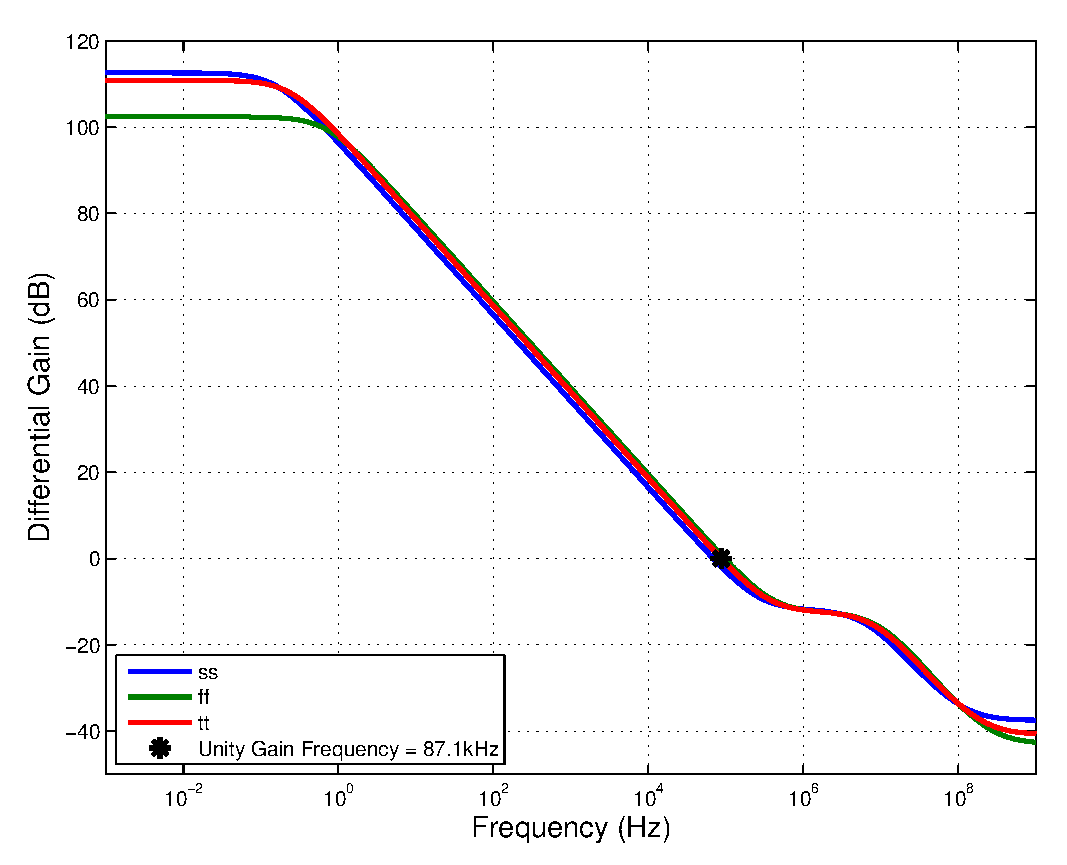
\includegraphics[width=4in]{Plots/open_dm_gain.eps}
\caption{The open loop differential gain magnitude response of the OTA.}
\label{fig:open_dm_gain}
\end{figure}


Open Loop Differential Phase Responses
\begin{figure}
\centering
\includegraphics[width=4in]{Plots/open_dm_phase.eps}
\caption{The open loop differential gain phase response of the OTA.}
\label{fig:open_dm_phase}
\end{figure}

\subsection{Open Loop Common Frequency Mode Response}

Open Loop Common Mode Magnitude Response
\begin{figure}
\centering
\includegraphics[width=4in]{Plots/open_cm_gain.eps}
\caption{The open loop common mode gain magnitude response of the OTA.}
\label{fig:open_cm_gain}
\end{figure}

Open Loop Common Mode Phase Response
\begin{figure}
\centering
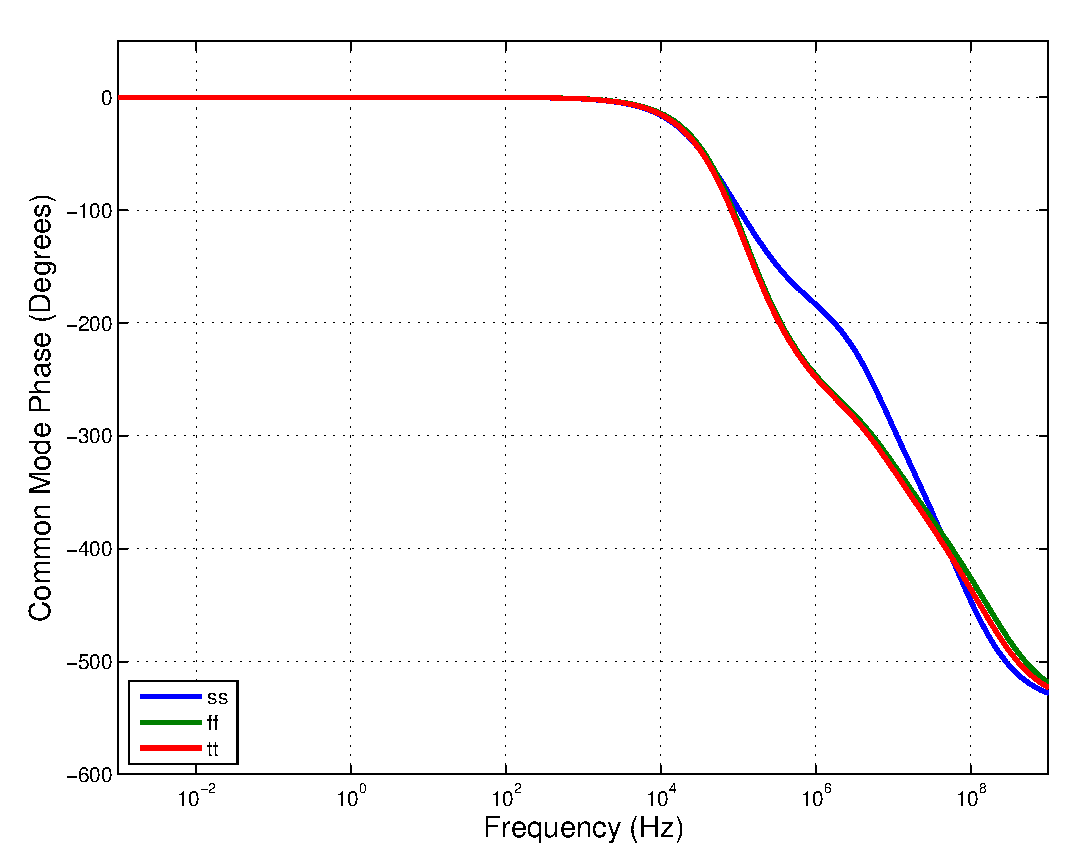
\includegraphics[width=4in]{Plots/open_cm_phase.eps}
\caption{The open loop common mode gain phase response of the OTA.}
\label{fig:open_cm_phase}
\end{figure}

\section{Closed Loop Amplifier Results}

\subsection{Nyquist Rate Sinusoidal Transient Response}

\begin{figure}
\centering
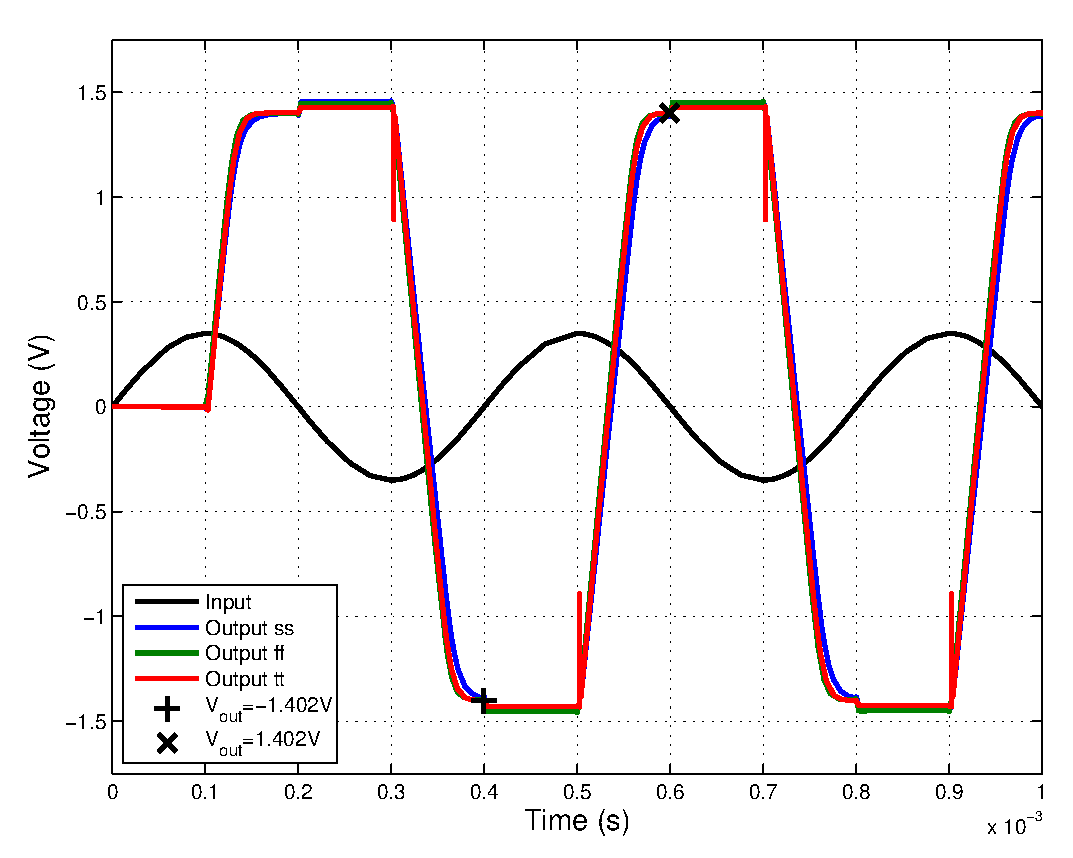
\includegraphics[width=4in]{Plots/closed_sine.eps}
\caption{The closed loop transient response to a full-scale amplitude sinusoid at the Nyquist frequency.}
\label{fig:closed_sine}
\end{figure}


\subsection{Small Step Transient Response}
\begin{figure}
\centering
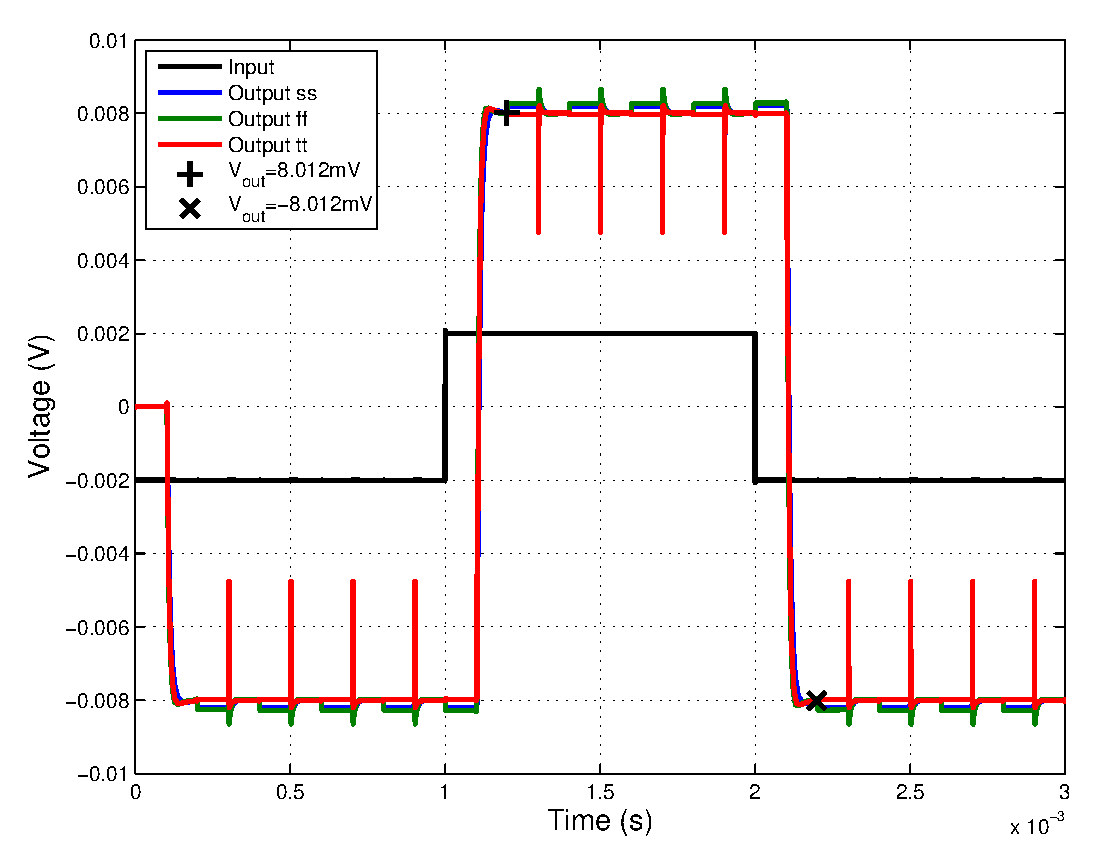
\includegraphics[width=4in]{Plots/closed_small_step.eps}
\caption{The closed loop transient response to a small amplitude step input.}
\label{fig:closed_small_step}
\end{figure}


\subsection{Full Scale Step Transient Response}
\begin{figure}
\centering
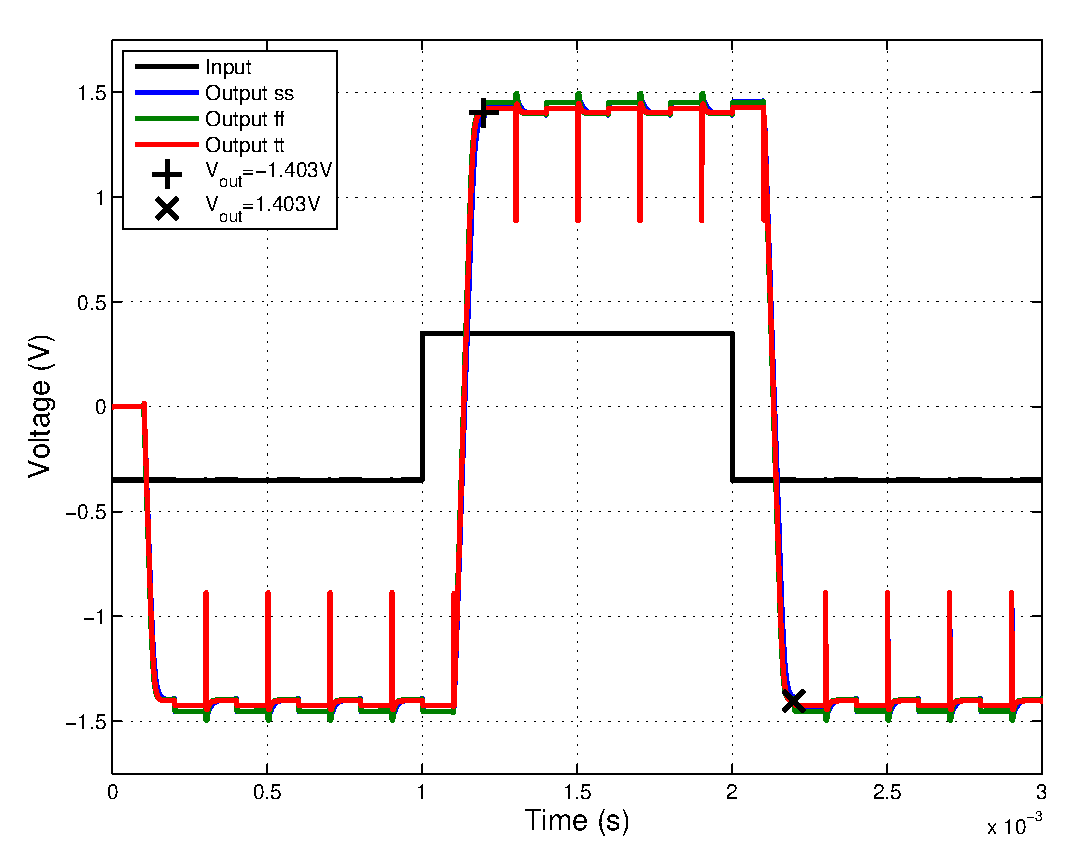
\includegraphics[width=4in]{Plots/closed_large_step.eps}
\caption{The closed loop transient response to a full-scale amplitude step input.}
\label{fig:closed_large_step}
\end{figure}

\subsection{Sawtooth Transient Response}
\begin{figure}
\centering
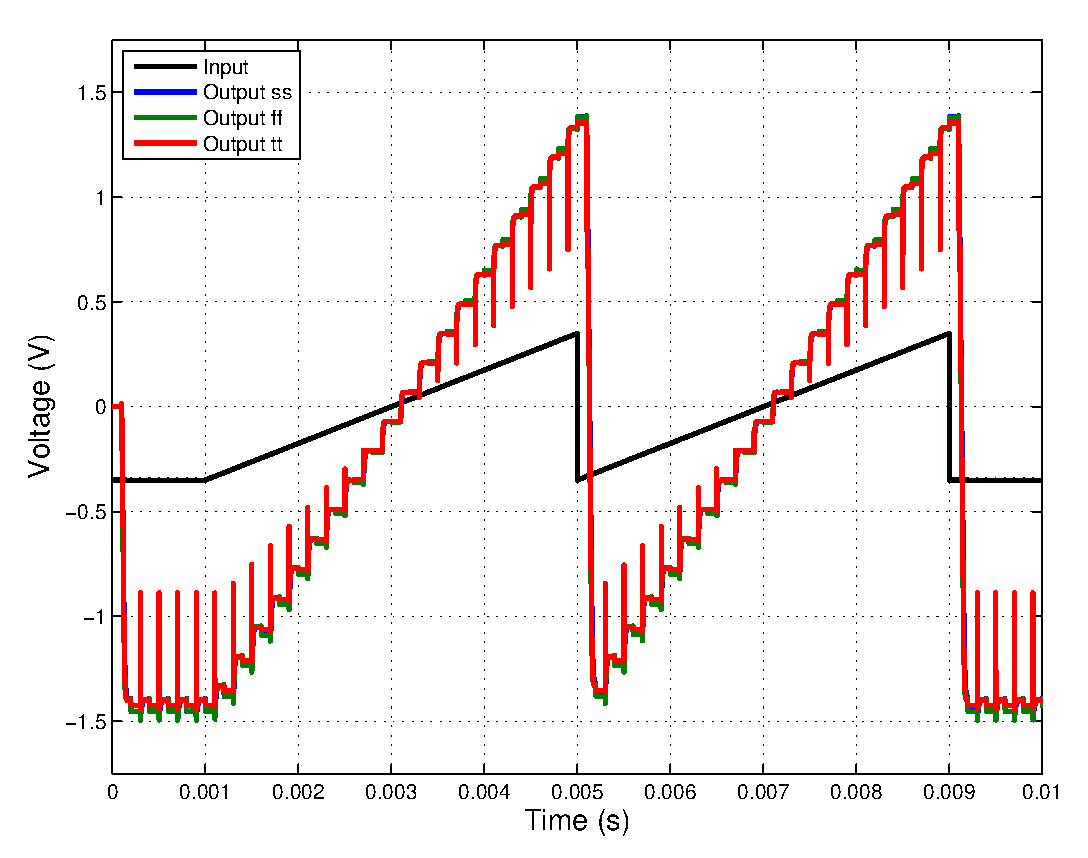
\includegraphics[width=4in]{Plots/closed_saw.eps}
\caption{The closed loop transient response to a full-scale amplitude sawtooth with a frequency of $\frac{f_s}{20}$.}
\label{fig:closed_saw}
\end{figure}

\subsection{Effective Number of Bits}

\subsection{Figure of Merit}

\subsection{Area}
transistor area

resistor area

capacitor area

total area

\section{Summary of Results}

\begin{table}
\centering
\caption{Summary of Specifications and Results}
\label{tab:specs_results}
\begin{tabular}{|c|c|c|c|c|}
\hline Specification & Specification Value & FF Result & TT Result & SS Result\\ 
\hline Open Loop OTA DC Gain &  & &  & \\ 
\hline Open Loop OTA Phase Margin &  & &  & \\ 
\hline Open Loop OTA $3dB$ Bandwidth &  & &  & \\ 
\hline Open Loop OTA Unity Gain Bandwidth &  & &  & \\ 
\hline Overall Power Consumption &  & &  & \\ 
\hline Overall Figure of Merit &  & &  & \\ 
\hline Overall Area &  & &  & \\ 
\hline  &  & &  & \\ 
\hline 
\end{tabular} 
\end{table}


\section{Possible Improvements}

\section{Conclusion}


% references section

% can use a bibliography generated by BibTeX as a .bbl file
% BibTeX documentation can be easily obtained at:
% http://www.ctan.org/tex-archive/biblio/bibtex/contrib/doc/
% The IEEEtran BibTeX style support page is at:
% http://www.michaelshell.org/tex/ieeetran/bibtex/
%\bibliographystyle{IEEEtran}
% argument is your BibTeX string definitions and bibliography database(s)
%\bibliography{IEEEabrv,../bib/paper}
%
% <OR> manually copy in the resultant .bbl file
% set second argument of \begin to the number of references
% (used to reserve space for the reference number labels box)
%%\begin{thebibliography}{1}
%%
%%\bibitem{sedrasmith}
%%A.~Sedra and K.~Smith, \emph{Microelectronic Circuits}, 6th~ed. \\ 
%%Oxford University Group, 2009. pgs. 711-716.  
%%\bibitem{LowGroupDelay}
%%Kim, J.; Buckwalter, J.F.; "Bandwidth Enhancement With Low Group-Delay Variation for a 40-Gb/s Transimpedance Amplifier," \emph{Circuits and Systems I: Regular Papers, IEEE Transactions on} , vol.57, no.8, pp.1964-1972, Aug. 2010.
%%
%%\end{thebibliography}

%\bibliographystyle{plain}
%\bibliography{AnalogProjectReferences}

\end{document}